\section{洛伦兹变换}\label{sec:11.04}

从速度合成律的讨论已经看到,光速不变原理与伽利略变换
是矛盾的。为了满足光速不变原理的要求,惯性系之间应当有不
同于式\eqref{eqn:11.02.02}的时空坐标变换关系,现在我们就来寻求它。

图11.1给出的两个惯性系$ K $及$ K' $,设在某一时刻(取为$ t = t ^ { \prime }
  =0 $),$ K $与$ K' $的原点是重合的,并且在这时刻位于原点的光源放
出一个光讯号。在$ K $中,光讯号的波前是以$ K $的原点为心的球
面,由下列方程所规定
\begin{equation*}
  x ^ { 2 } + y ^ { 2 } + z ^ { 2 } - c ^ { 2 } t ^ { 2 } = 0
\end{equation*}

\begin{figure}[h]
  \centering
  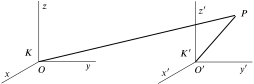
\includegraphics{figure/fig11.01}
  \caption{$ K $及$ K' $两个参考系}
  \label{fig:11.01}
\end{figure}
由于光速不变,在$ K' $中,这个光讯号的波前应是以$ K' $的原点为
% 325.jpg
心的球面,即
\begin{equation*}
  x ^ { \prime 2 } + y ^ { \prime 2 } + t ^ { \prime 2 } - c ^ { 2 } t ^ { \prime 2 } = 0
\end{equation*}
这样,只要要求$ \left( x , y , z , t \right) $与$ \left( x ^ { \prime } , y ^ { \prime } , z ^ { \prime } , t ^ { \prime } \right) $之间的变换关系
满足下式\vspace{-1.4em}
\begin{equation}\label{eqn:11.04.01}
  \begin{split}
    &x ^ { 2 } + y ^ { 2 } + z ^ { 2 } - c ^ { 2 } t ^ { 2 } \\[-0.3em]
    = &x ^ { \prime 2 } + y ^ { \prime 2 } + z ^ { \prime 2 } - c ^ { 2 } t ^ { \prime 2 }
  \end{split}
\end{equation}
就可以与光速不变原理相适应。

现在我们来求满足式\eqref{eqn:11.04.01}的坐标变换关系。首先我们注
意到,因为只在$ x $方向$ K $与$ K' $有相对运动,$ y , z $方向并没有相对
运动,所以关于$ y , z $的变换应当是
\begin{equation}\label{eqn:11.04.02}
  y ^ { \prime } = y \qquad z ^ { \prime } = z
\end{equation}
另外,还应要求坐标变换是线性的,这个要求来源于空间的均匀
性,即空间中各点的性质都是一样的,没有任何具有特别性质的
点。这样,$ x, t $与$ x ^ { \prime }, t ^ { \prime } $之间的关系应有下列的一般形式:
\begin{equation}\label{eqn:11.04.03}
  \begin{split}
    x ^ { \prime } &= \alpha x + \gamma t \\[-0.3em]
    t ^ { \prime } &= \delta x + \eta t
  \end{split}
\end{equation}
为了使式\eqref{eqn:11.04.03}满足于式\eqref{eqn:11.04.01},即
\begin{equation}\label{eqn:11.04.04}
  x ^ { 2 } - c ^ { 2 } t ^ { 2 } = x ^ { \prime 2 } - c ^ { 2 } t ^ { \prime 2 }
\end{equation}
式\eqref{eqn:11.04.03}应具有下列形式:
\begin{equation}\label{eqn:11.04.05}
  \begin{split}
    x ^ { \prime } &= x \ch \theta - c t \sh \theta \\[-0.3em]
    c t ^ { \prime } &= - x \sh \theta + c t \ch \theta
  \end{split}
\end{equation}
其中$\theta$为常量。容易验证式\eqref{eqn:11.04.05}符合式\eqref{eqn:11.04.04}:
\begin{equation*}
  \begin{split}
    &x ^ { \prime 2 } - c ^ { 2 } t ^ { \prime 2 } \\[-0.3em]
    =& \left( x \ch \theta - c t \sh \theta \right) ^ { 2 } - \left( - x \sh \theta + c t \ch \theta \right) ^ { 2 } \\[-0.3em]
    =& x ^ { 2 } \left( \ch ^ { 2 } \theta - \sh ^ { 2 } \theta \right) - c ^ { 2 } t ^ { 2 } \left( \ch ^ { 2 } \theta - \sh ^ { 2 } \theta \right) \\[-0.3em]
    =& x ^ { 2 } - c ^ { 2 } t ^ { 2 }
  \end{split}
\end{equation*}
引入新参数\vspace{-1.8em}
\begin{equation*}
  \beta = \tgh \theta
\end{equation*}

% 326.jpg
\begin{align*}
  \beforetext{亦即} \sh \theta = \frac { \beta } { \sqrt { 1 - \beta ^ { 2 } } } \qquad
  \ch \theta = \frac { 1 } { \sqrt { 1 - \beta ^ { 2 } } }
\end{align*}
式\eqref{eqn:11.04.05}还可以改写成
\begin{equation}\label{eqn:11.04.06}
  \begin{split}
    x ^ { \prime } &= \frac { x - \beta c t } { \sqrt { 1 - \beta ^ { 2 } } } \\
    t ^ { \prime } &= \frac { t - \beta \dfrac x c } { \sqrt { 1 - \beta ^ { 2 } } }
  \end{split}
\end{equation}
或者把\eqref{eqn:11.04.02}及\eqref{eqn:11.04.06}的$ x, y, z, t $解出,得到
\begin{equation}\label{eqn:11.04.07}
  \begin{split}
    x &= \frac { x ^ { \prime } + \beta c ^ { \prime } } { \sqrt { 1 - \beta ^ { 2 } } } \\
    y &= y ^ { \prime } \\
    z &= z ^ { \prime } \\[-0.5em]
    t &= \frac { t ^ { \prime } + \beta \dfrac { x ^ \prime } { c } } { \sqrt { 1 - \beta ^ { 2 } } }
  \end{split}
\end{equation}
现在,我们来确定系数$\beta$。由于$ K' $相对于$ K $在$ x $方向以速度$ v $运
动,所以对于$ K $中的观察者,$ K' $的原点,即$ x ^ { \prime } = y ^ { \prime } = z ^ { \prime } = 0 $点的速
度应是$ \dfrac { \dif x } { \dif t } = v, \dfrac { \dif y } { \dif t } = 0, \dfrac { \dif z } { \dif t } = 0 $。另一方面由式\eqref{eqn:11.04.07}可得
(注意用$ x ^ { \prime } = y ^ { \prime } = z ^ { \prime } = 0 $):
\begin{equation*}
  \dif x = \frac { \beta c \dif t ^ { \prime } } { \sqrt { 1 - \beta ^ { 2 } }} \quad \dif y = 0 \quad \dif z = 0 \quad \dif t = \frac { \dif t ^ { \prime } } { \sqrt { 1 - \beta ^ { 2 } } }
\end{equation*}
\begin{align*}
  \beforetext{故}\frac { \dif x } { \dif t } = \frac { \beta c \sqrt { 1 - \beta ^ { 2 } } } { \sqrt { 1 - \beta ^ { 2 } } } = \beta c \quad \frac { \dif y } { \dif t } = \frac { \dif z } { \dif t } = 0
\end{align*}
所以得到
\begin{equation}\label{eqn:11.04.08}
  \beta c = v \quad \beta = \frac v c
\end{equation}
% 327.jpg
将上式代入式\eqref{eqn:11.04.02}、\eqref{eqn:11.04.06}或者式\eqref{eqn:11.04.07},就得到惯性
系$ K $与$ K' $之间的时空坐标变换关系
\begin{equation}\label{eqn:11.04.09}
  \begin{cases}
    x ^ { \prime } = \dfrac { x - v t } { \sqrt { 1 - v ^ 2 / c ^ 2 } } \\
    y ^ { \prime } = y                                                  \\
    z ^ { \prime } = z                                                  \\
    t ^ { \prime } = \dfrac { t - \dfrac v { c ^ 2 } x } { \sqrt { 1 - v ^ 2 / c ^ 2 } }
  \end{cases}
\end{equation}
或
\begin{equation}\label{eqn:11.04.10}
  \begin{cases}
    x = \dfrac { x ^ { \prime } + v t ^ { \prime } } { \sqrt { 1 - v ^ 2 / c ^ 2 } } \\
    y = y ^ { \prime }                                                               \\
    z = z ^ { \prime }                                                               \\
    t = \dfrac { t ^ { \prime } + \dfrac v { c ^ 2 } x ^ { \prime } } { \sqrt { 1 - v ^ 2 / c ^ 2 } }
  \end{cases}
\end{equation}
式\eqref{eqn:11.04.09}或\eqref{eqn:11.04.10}称为\CJKunderdot{洛伦兹}变换。

当速度$ v \ll c $即$ \dfrac { v ^ { 2 } } { c ^ { 2 } } \ll 1 $时,如果忽略掉
$ \beta ^ { 2 } = \left( \dfrac { v } { c } \right) ^ { 2 } $
以上的各级
小量,式\eqref{eqn:11.04.09}就过渡为伽利略变换\lhbrak 式\eqref{eqn:11.02.02}\rhbrak 了。这表明,
在牛顿力学中所采用的时空坐标变换是只适用于低速情况的,在
高速情况它不正确。

在伽利略变换中,时间与空间是相互分开的,变换$ t ^ { \prime } = t + t _ { 0 } $
中只含有$ K $及$ K ' $中的时间坐标。这正符合我们按日常经验所建
立
起来的观念:时间与空间是“绝对”分开的两个概念。但是,在
洛伦兹变换\lhbrak 式\eqref{eqn:11.04.09}\rhbrak 中,时间的变换不再与空间无关。
